\chapter{Introduction} \label{sectionIntroduction}

We have several areas of concern when building software systems: cost, delivery timeline, and quality. The cost and time-to-market are often the two problems given the highest priority in a project. However, engineers must consider the software quality to preserve the system's longevity. Despite their importance, the code and architecture quality can be challenging to understand and measure.

The art of programming began as something very tedious and error-prone, with developers writing every step of a process in a machine language. As writing machine code was not a great way to grow the industry, developers created programming languages. With human-friendly languages, programmers could reduce the manual effort in writing code and improve the quality of their work by allowing the machine to transform the high-level code into something executable and efficient. \cite{lehman:1980}

With the creation of programming languages, the ability to build systems and applications has become a skill that almost anyone can learn. Open source projects create communities of learning and advancement. However, all systems need structure and an investment of time.

When we think about programming projects, we can assume that as time goes on and changes and additions occur within a system's source code, the complexity of that system will grow. However, when we manage the code structure, we can keep the complexity in check, allowing systems to evolve. For example, developers can maintain this structure through simple steps like having readable code. They can also consider more complex aspects, like how coupled and cohesive a system is.

One way to understand the quality of a system is to discuss its ``maintainability,'' the ease of receiving new features or resolving bugs. Such as, developers may find that adjusting one area to add a new feature requires touching several other code areas in tightly coupled systems. Some code measuring systems provide a Maintainability Index (MI), a well-known quality measure. While the effectiveness of quantifying software quality is debatable, many quality models include MI measurements \cite{vandeursen:2014}, \cite{adewumi:2016}. 

Adewumi et al. found that 55\% of the existing Open Source Software (OSS) quality models measure maintainability, making it the most common quality characteristic measured \cite{adewumi:2016}. From ``Fig.~\ref{figFreqDistProductQualityModel},'' we can infer that maintainability is more important than functional stability. If the code is maintainable and accessible, missing features can be incorporated. However, it would be hard to implement if the code is not well documented and is difficult to read and understand \cite{adewumi:2016}.

\begin{figure}[ht]
  \centerline{
      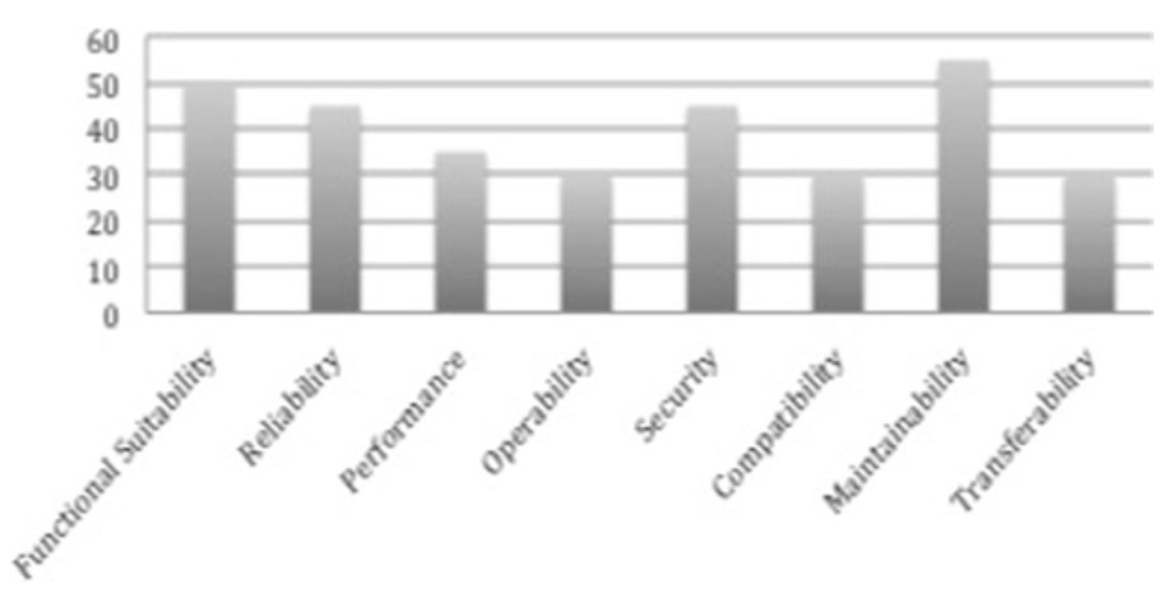
\includegraphics[width=0.7\columnwidth]{adewole_ProductQualityCharacteristics_in_OSS_quality_models.png}
  }
  \caption{Frequency distribution of ISO 25010 product quality characteristics in OSS quality models, as found by Adewumi et al. in 2016 \cite{adewumi:2016}.}
  \label{figFreqDistProductQualityModel}
\end{figure}

Code smells are used extensively by practitioners to identify low-quality spots in the software system. These areas would need the teams' attention and are good candidates for refactoring. Rather than building comprehensive models with all possible software characteristics, developers should instead focus on the essential characteristics: maintainability, usability, and maintenance capacity of a software community \cite{adewumi:2016}.
